\chapter{Fonctions usuelles}
\def\arraystretch{1}

\begin{definition}[Fonction polynomiale]
	Soient $n \in \N$ et $a_i \in \R$.
	\begin{center}
		$
		\appli{f}{\R}{\R}{x}{\sum_{i=0}^n a_i x^i}
		$
	\end{center}
\end{definition}

\begin{definition}[Fonction partie entière]
	\[ \forall x \in \R,\ \exists ! E(x) \in \Z,\ E(x) \leq x < E(x + 1) \]
	\begin{center}
		$
		\appli{E}{\R}{\Z}{x}{E(x)}
		$
	\end{center}
	Parfois la partie entière est notée $\floor{x}$.
\end{definition}

\begin{figure}[!h]
	\centering
	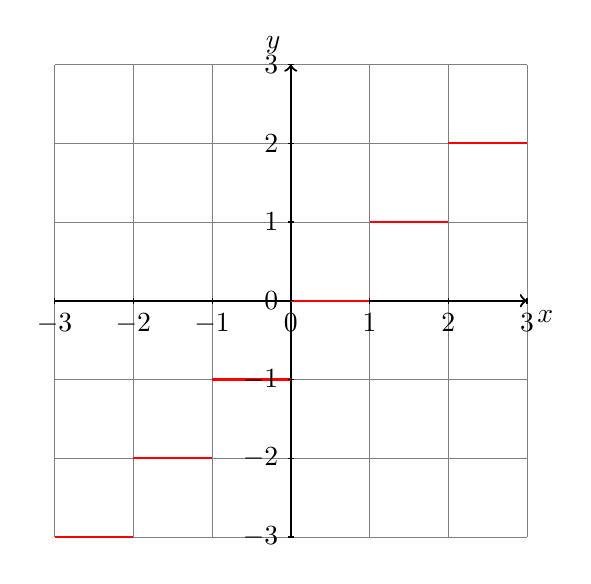
\begin{tikzpicture}
		\draw[step=1cm, gray, very thin] (-3, -3) grid (3, 3);
		\draw[thick, ->] (-3, 0) -- (3, 0) node[anchor=north west] {$x$};
		\draw[thick, ->] (0, -3) -- (0, 3) node[anchor=south east] {$y$};
		\draw[thick, red] (1, 1) -- (2, 1);
		\draw[thick, red] (2, 2) -- (3, 2);
		\draw[thick, red] (0, 0) -- (1, 0);
		\draw[thick, red] (-1, -1) -- (0, -1);
		\draw[thick, red] (-2, -2) -- (-1, -2);
		\draw[thick, red] (-3, -3) -- (-2, -3);
		\foreach \x in {-3, -2, -1, 0, 1, 2, 3}
			\draw (\x cm, 1pt) -- (\x cm, -1pt) node[anchor=north] {$\x$};
		\foreach \y in {-3, -2, -1, 0, 1, 2, 3}
			\draw (1pt, \y cm) -- (-1pt, \y cm) node[anchor=east] {$\y$};
	\end{tikzpicture}
	\caption{Graphe de la fonction partie entière}
\end{figure}

\begin{definition}[Fonction puissance]
	Soit $a \in \R$.
	\begin{center}
		$
		\appli{f}{\R_+^*}{\R}{x}{x^a}
		$
	\end{center}
\end{definition}

\begin{proposition}
	Soient $a, b, x \in \R$.
    \begin{enumerate}
            \item $1^a = 1$.
            \item $x^0 = 1$.
            \item $x^a \cdot x^b = x^{a + b}$.
            \item Si $x \neq 0$ alors :
            \begin{enumerate}
            	\item $\frac{1}{x^a} = x^{-a}$.
            	\item $\frac{x^a}{x^b} = x^{a - b}$.
            \end{enumerate}
            \item $(xy)^a = x^a y^a$.
            \item $(x^a)^b = x^{ab}$.
        \end{enumerate}
\end{proposition}

\begin{proposition}
	La dérivée de la fonction $x^a$ est $ax^{a-1}$.
\end{proposition}

\begin{proof}
	Dans le cas où la puissance est un entier naturel. \\
	Procèdons par récurrence pour montrer $P_n : (x^n)' = nx^{n-1}$.
	\begin{enumerate}
		\item \textbf{Initialisation :} En $n = 0$, $f_0(x) = 1$ donc :
		\begin{align*}
			f_0'(a) &= \lim_{x \to a} \frac{f_0(x) - f_0(a)}{x - a} \\
			 &= \lim_{x \to a} \frac{1 - 1}{x - a} \\
			 &= 0
		\end{align*}
		En $n = 1$, $f_1(x) = x$ donc :
		\begin{align*}
			f_1'(a) &= \lim_{x \to a} \frac{x - a}{x - a} = 1
		\end{align*}
		\item \textbf{Hérédité :} On suppose que $P_k$ est vraie pour un $k > 2$. \\
		On a : $f_{k+1}'(x) = (x - x^k)' = (f_1(x) f_k(x))'$.
		\begin{align*}
			f_{k+1}'(x) &= f_1'(x) f_k(x) + f_1(x) f_n'(x) \\
			&= x^k + xkx^{k-1} \\
			&= (k+1)x^k 
		\end{align*}
	\end{enumerate}
\end{proof}

\section{Fonctions trigonométriques}
\begin{definition}[Fonctions trigonométriques]
	Soit $k \in \Z$ :	
	\begin{center}
		$
		\begin{array}{ccc}
			\appli{\cos}{\R}{[-1,1]}{x}{\cos(x)}
			&
			\appli{\sin}{\R}{[-1,1]}{x}{\sin(x)}
			&
			\appli{\tan}{\R \backslash \left\{ \frac{k \pi}{2} \right\}}{\R}{x}{\frac{\sin(x)}{\cos(x)}}
		\end{array}
		$
	\end{center}	
\end{definition}

\begin{proposition}
	Soient $x \in \R$ et $k \in \Z$.
	\begin{enumerate}
		\item $\cos(-x) = \cos(x)$.
		\item $\sin(-x) = -\sin(x)$.
		\item $\tan(-x) = -\tan(x)$.
		\item $\cos(x + 2k\pi) = \cos(x)$.
		\item $\sin(x + 2k\pi) = \sin(x)$.
		\item $\tan(x + k\pi) = \tan(x)$.
		\item $\cos$ est bijective sur $[0, \pi]$.
		\item $\sin$ est bijective sur $[-\frac{\pi}{2}, \frac{\pi}{2}]$.
		\item $\tan$ est bijective sur $]-\frac{\pi}{2}, \frac{\pi}{2}[$.
	\end{enumerate}
\end{proposition}

\begin{figure}[h!]
	\centering
	%\includegraphics{images/cos.png}
	\begin{subfigure}{0.3\textwidth}
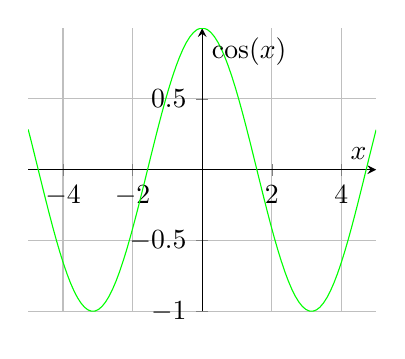
\begin{tikzpicture}
            \begin{axis}[domain=-5:5, axis lines=middle, grid=both, xlabel=$x$, ylabel=$\cos(x)$, width=6cm]
                \addplot[color=green, samples=100] {cos(deg(x))};
            \end{axis}
    \end{tikzpicture}
		
		\caption{Fonction $\cos{x}$}
	\end{subfigure}
	\begin{subfigure}{0.3\textwidth}
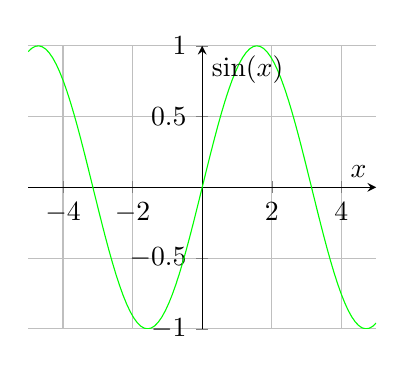
\begin{tikzpicture}
            \begin{axis}[domain=-5:5, axis lines=middle, grid=both, xlabel=$x$, ylabel=$\sin(x)$, width=6cm]
                \addplot[color=green, samples=100] {sin(deg(x))};
            \end{axis}
    \end{tikzpicture}
		\caption{Fonction $\sin{x}$}
	\end{subfigure}
	\begin{subfigure}{0.3\textwidth}
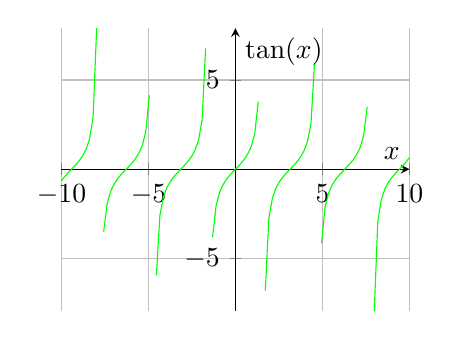
\begin{tikzpicture}
            \begin{axis}[domain=-10:10, restrict y to domain=-10:10, axis lines=middle, grid=both, xlabel=$x$, ylabel=$\tan(x)$, width=6cm]
                \addplot[color=green, samples=100] {tan(deg(x))};
            \end{axis}
    \end{tikzpicture}
		\caption{Fonction $\tan{x}$}
	\end{subfigure}
\end{figure}

\begin{figure}[h!]
	\centering
	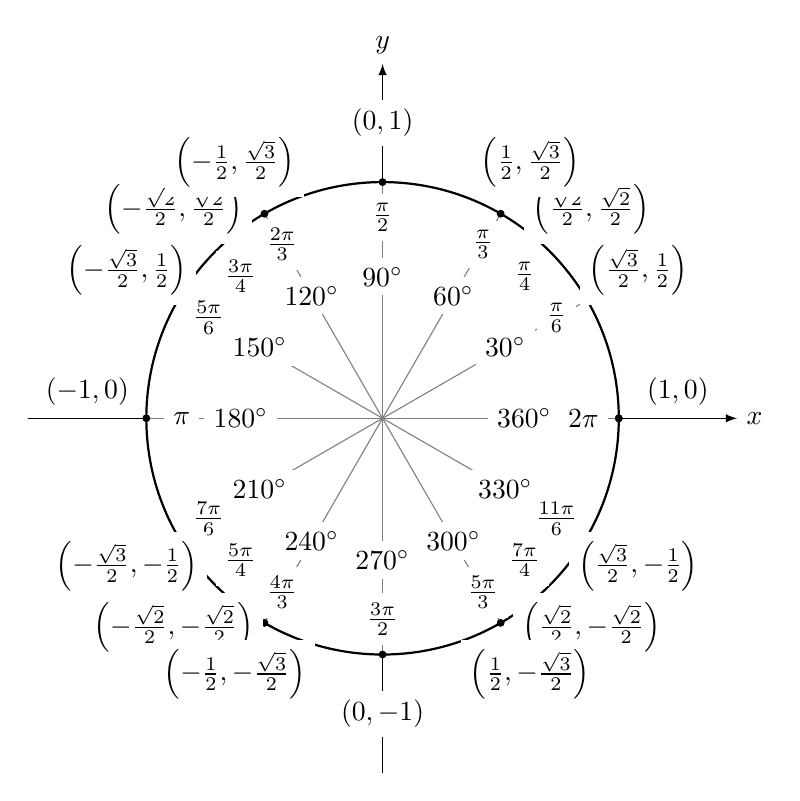
\begin{tikzpicture}[scale=3,cap=round,>=latex]
		% draw the coordinates
		\draw[->] (-1.5cm,0cm) -- (1.5cm,0cm) node[right,fill=white] {$x$};
		\draw[->] (0cm,-1.5cm) -- (0cm,1.5cm) node[above,fill=white] {$y$};
		
		% draw the unit circle
		\draw[thick] (0cm,0cm) circle(1cm);
		
		\foreach \x in {0,30,...,360} {
			% lines from center to point
			\draw[gray] (0cm,0cm) -- (\x:1cm);
			% dots at each point
			\filldraw[black] (\x:1cm) circle(0.4pt);
			% draw each angle in degrees
			\draw (\x:0.6cm) node[fill=white] {$\x^\circ$};
		}
		
		% draw each angle in radians
		\foreach \x/\xtext in {
			30/\frac{\pi}{6},
			45/\frac{\pi}{4},
			60/\frac{\pi}{3},
			90/\frac{\pi}{2},
			120/\frac{2\pi}{3},
			135/\frac{3\pi}{4},
			150/\frac{5\pi}{6},
			180/\pi,
			210/\frac{7\pi}{6},
			225/\frac{5\pi}{4},
			240/\frac{4\pi}{3},
			270/\frac{3\pi}{2},
			300/\frac{5\pi}{3},
			315/\frac{7\pi}{4},
			330/\frac{11\pi}{6},
			360/2\pi}
		\draw (\x:0.85cm) node[fill=white] {$\xtext$};
		
		\foreach \x/\xtext/\y in {
			% the coordinates for the first quadrant
			30/\frac{\sqrt{3}}{2}/\frac{1}{2},
			45/\frac{\sqrt{2}}{2}/\frac{\sqrt{2}}{2},
			60/\frac{1}{2}/\frac{\sqrt{3}}{2},
			% the coordinates for the second quadrant
			150/-\frac{\sqrt{3}}{2}/\frac{1}{2},
			135/-\frac{\sqrt{2}}{2}/\frac{\sqrt{2}}{2},
			120/-\frac{1}{2}/\frac{\sqrt{3}}{2},
			% the coordinates for the third quadrant
			210/-\frac{\sqrt{3}}{2}/-\frac{1}{2},
			225/-\frac{\sqrt{2}}{2}/-\frac{\sqrt{2}}{2},
			240/-\frac{1}{2}/-\frac{\sqrt{3}}{2},
			% the coordinates for the fourth quadrant
			330/\frac{\sqrt{3}}{2}/-\frac{1}{2},
			315/\frac{\sqrt{2}}{2}/-\frac{\sqrt{2}}{2},
			300/\frac{1}{2}/-\frac{\sqrt{3}}{2}}
		\draw (\x:1.25cm) node[fill=white] {$\left(\xtext,\y\right)$};
		
		% draw the horizontal and vertical coordinates
		% the placement is better this way
		\draw (-1.25cm,0cm) node[above=1pt] {$(-1,0)$}
		(1.25cm,0cm)  node[above=1pt] {$(1,0)$}
		(0cm,-1.25cm) node[fill=white] {$(0,-1)$}
		(0cm,1.25cm)  node[fill=white] {$(0,1)$};
	\end{tikzpicture}
	\caption{Cercle trigonométrique}
\end{figure}

\begin{proposition}
	\begin{enumerate}
		\item $\cos'(x) = -\sin(x)$. 
		\item $\sin'(x) = \cos(x)$.
		\item $\tan'(x) = \frac{1}{\cos^2(x)} = 1 + \tan^2(x)$.
	\end{enumerate}
\end{proposition}

\begin{proof}
	Montrons le 3.
	On part de $\tan(x) = \frac{\sin(x)}{\cos(x)}$.
	\begin{align*}
		\left( \frac{\sin(x)}{\cos(x)} \right) &= \frac{\sin'(x) \cos(x) - \sin(x) \cos'(x)}{\cos^2(x)} \\
		&= \frac{\cos^2(x) + \sin^2(x)}{\cos^2(x)}
	\end{align*}
	On peut simplifier le résultat de deux manières :
	\begin{enumerate}
		\item On peut utiliser $\cos^2(x) + \sin^2(x) = 1$
		donc on aurait :
		\[ \tan'(x) = \frac{1}{\cos^2(x)} \]
		\item On peut aussi séparer la fraction en deux :
		\begin{align*}
			\tan'(x) &= \frac{\cos^2(x)}{\cos^2(x)} + \frac{\sin^2(x)}{\cos^2(x)} \\
			&= 1 + \left( \frac{\sin(x)}{\cos(x)} \right)^2 \\
			&= 1 + \tan^2(x)
		\end{align*}
	\end{enumerate}
\end{proof}

\begin{definition}
	On définit $\arccos,\ \arcsin$ et $\arctan$ comme étant les bijections réciproques des fonctions $\cos,\ \sin$ et $\tan$.
\end{definition}

\begin{figure}[h!]
	\centering
	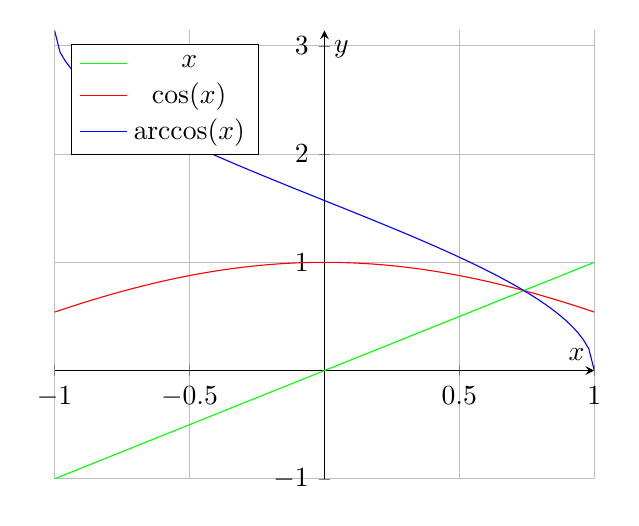
\begin{tikzpicture}
		\begin{axis}[domain=-1:1, axis lines=middle, grid=both, xlabel=$x$, ylabel=$y$, samples=100, legend pos=north west]
			\addplot[color=green]{x};
			\addlegendentry{$x$}
			\addplot[color=red]  {cos(deg(x))};
			\addlegendentry{$\cos(x)$}
			\addplot[color=blue]  {rad(acos(x))};
			\addlegendentry{$\arccos(x)$}
		\end{axis}
	\end{tikzpicture}
	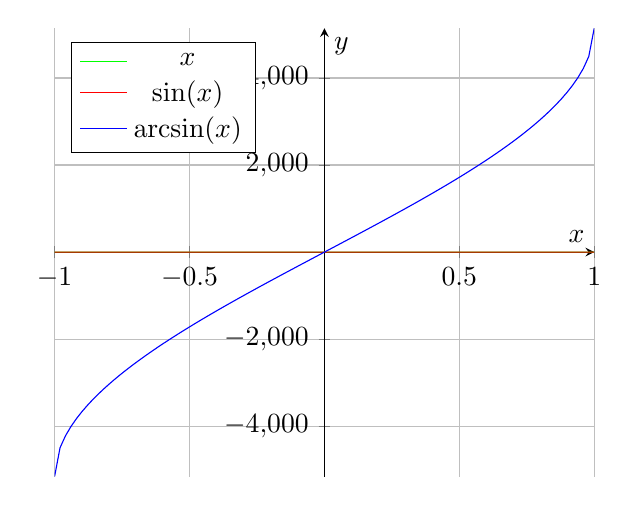
\begin{tikzpicture}
		\begin{axis}[domain=-1:1, axis lines=middle, grid=both, xlabel=$x$, ylabel=$y$, samples=100, legend pos=north west]
			\addplot[color=green]{x};
			\addlegendentry{$x$};
			\addplot[color=red]  {sin(deg(x))};
			\addlegendentry{$\sin(x)$};
			\addplot[color=blue]  {deg(asin(x))};
			\addlegendentry{$\arcsin(x)$};
		\end{axis}
	\end{tikzpicture}
	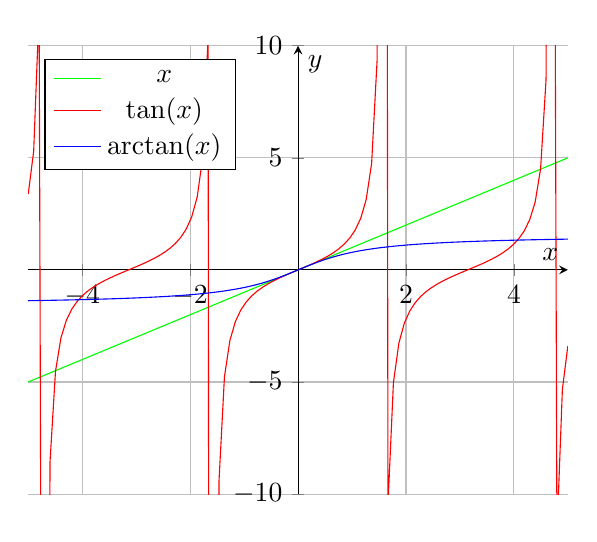
\begin{tikzpicture}
		\begin{axis}[xmin=-5, xmax=5, ymin=-10, ymax=10, axis lines=middle, grid=both, xlabel=$x$, ylabel=$y$, samples=100, legend pos=north west]
			\addplot[color=green]{x};
			\addlegendentry{$x$};
			\addplot[color=red]  {tan(deg(x))};
			\addlegendentry{$\tan(x)$};
			\addplot[color=blue]  {rad(atan(x))};
			\addlegendentry{$\arctan(x)$};
		\end{axis}
	\end{tikzpicture}
\end{figure}

\begin{proposition}
    \begin{enumerate}
    	\item $\forall x \in [-\frac{\pi}{2}, \frac{\pi}{2}] : \arcsin(\sin(x)) = x$.
        \item $\forall x \in ]-\frac{\pi}{2}, \frac{\pi}{2}[ ! \arctan(\tan(x)) = x$.
        \item $\forall x \in [0, \pi] : \arccos(\cos(x)) = x$.
        \item $\forall x \in [-1, 1]$ :
        \begin{enumerate}
                \item $\sin(\arcsin(x)) = x$.
                \item $\cos(\arccos(x)) = x$.
            \end{enumerate}
        \item $\forall x \in \R : \tan(\arctan(x)) = x$.
    \end{enumerate}
\end{proposition}

\begin{proposition}
	Soient $a, b \in \R$.
        \begin{enumerate}
            \item $\sin(a + b) = \sin(a) \cos(b) + \sin(b) \cos(a)$.
            \item $\cos(a + b) = \cos(a) \cos(b) - \sin(a) \sin(b)$.
        \end{enumerate}
\end{proposition}

\begin{proof}
    Nous pouvons procéder avec des produits scalaires, mais nous allons utiliser les nombres complexes ici.
    \\
    D'une part :
    \[e^{i (a + b)} = \cos(a + b) + i\sin(a + b)\]
    D'autre part :
    \begin{align*}
        e^{i (a + b)} &= e^{ia} \cdot e^{ib} \\
        &= [\cos(a) + i \sin(a)] \cdot [\cos(b) + i \sin(b)] \\
        &= \cos(a) \cos(b) + i\sin(b)\cos(a) + i\sin(a)\cos(b) - \sin(a)\sin(b) \\
        &= \cos(a)\cos(b) - \sin(a)\sin(b) + i [\sin(b)\cos(a) + \sin(a) \cos(b)].
    \end{align*}
    Par identification de la partie réelle et de la partie imaginaire :
    \[ \sin(a + b) = \sin(a) \cos(b) + \sin(b) \cos(a) \]
	\[ \cos(a + b) = \cos(a) \cos(b) - \sin(a) \sin(b) \]
\end{proof}

\begin{proposition}
    Soit $x \in \R$.
    \[ \cos^2(x) + \sin^2(x) = 1 \]
\end{proposition}

\begin{proof}
    C'est une application du théorème de Pythagore sachant que le rayon du cercle trigonométrique est égal à 1.
\end{proof}

\begin{proposition}
    \begin{enumerate}
        \item $\lim_{x \to +\infty} \arctan(x) = \frac{\pi}{2}$.
        \item $\lim_{x \to -\infty} \arctan(x) = -\frac{\pi}{2}$.
    \end{enumerate}
\end{proposition}

\section{Exponentielle et logarithme}

\begin{theorem}[Fonction exponentielle]
	Il existe une unique fonction dérivable 
	\begin{center}
		$
		\appli{\exp}{\R}{\R_+^*}{x}{\exp(x) = e^x}
		$
	\end{center}
	telle que $\exp'(x) = \exp(x)$ et $\exp(0) = 1$.
\end{theorem}

\begin{proposition}
	La fonction exponentielle est \textbf{bijective} et \textbf{strictement croissante} et $\exp(0) = 1$.
    \begin{enumerate}
            \item $\lim_{x \to -\infty} e^x = 0$.
            \item $\lim_{x \to +\infty} e^x = +\infty$.
        \end{enumerate}
    \noindent Soient $x, y \in \R$.
    \begin{enumerate}
            \item $\exp(x + y) = \exp(x) \cdot \exp(y)$.
            \item $\exp(-x) = \frac{1}{\exp(x)}$.
            \item $\exp(x - y) = \frac{\exp(x)}{\exp(y)}$.
        \end{enumerate}
\end{proposition}

\begin{definition}[Logarithme néperien]
	\begin{center}
		$
		\appli{\ln}{\R_+^*}{\R}{x}{\ln(x)}
		$
	\end{center}
\end{definition}

\begin{figure}[!h]
	\centering
	\begin{subfigure}{0.45\textwidth}
		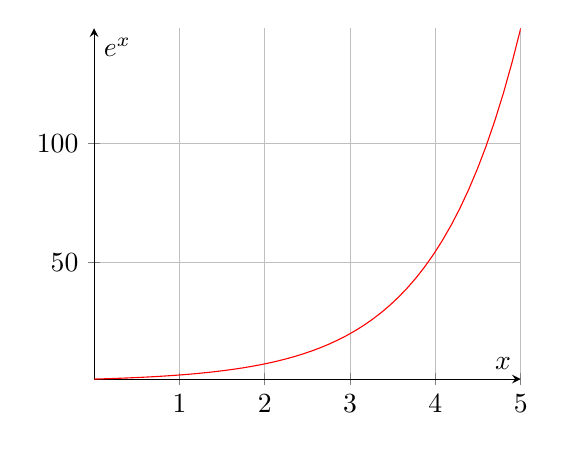
\begin{tikzpicture}
			\begin{axis}[domain=0:5, axis lines=middle, grid=both, xlabel=$x$, ylabel=$e^x$, width=7cm]
				\addplot[color=red, samples=50]{e^x};
			\end{axis}
		\end{tikzpicture}  
		\caption{Fonction exponentielle}
	\end{subfigure}
	\begin{subfigure}{0.45\textwidth}
		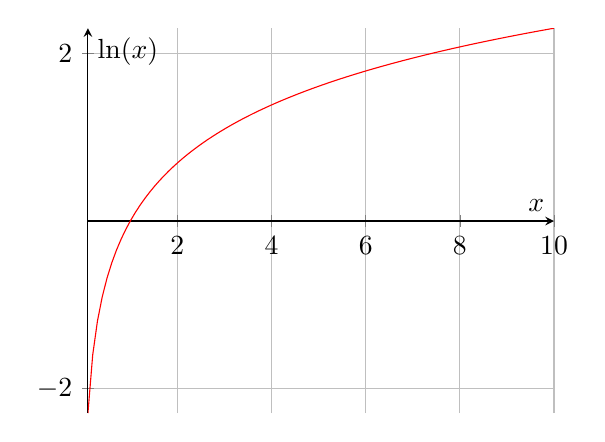
\begin{tikzpicture}
			\begin{axis}[domain=0:10, axis lines=middle, grid=both, xlabel=$x$, ylabel=$\ln(x)$, width=7.5cm]
				\addplot[color=red, samples=100]{ln(x)};
			\end{axis}
		\end{tikzpicture}
		\caption{Fonction logarithme népérien}
	\end{subfigure}
\end{figure}

\begin{proposition}
	Soient $x \in \R_+^*$ et $y \in \R$.
    \begin{multicols}{2}
        \begin{enumerate}
            \item $\exp(\ln(x)) = x$.
            \item $\ln(\exp(y)) = y$.
        \end{enumerate}
    \end{multicols}
\end{proposition}

\begin{proposition}
	Soit $x \in \R_+^*$.
	\[ \ln'(x) = \frac{1}{x} \]
\end{proposition}

\begin{proof}
	On utilise la propriété suivante pour $y \in \R$ : $\ln(\exp(y)) = y$.
	\begin{align*}
		&\ln(\exp(y)) = y \\
		&(\ln(\exp(y))' = y' \\
		&\ln'(\exp(y)) \exp'(y) = 1 \\
		&\ln'(\exp(y)) \exp(y) = 1 \\
		&\ln'(\exp(y)) = \frac{1}{\exp(y)}
	\end{align*}
	En posant $x = \exp(y)$ :
	\[ \ln'(x) = \frac{1}{x} \]
\end{proof}

\begin{proposition}
	La fonction logarithme néperien est \textbf{bijective} et \textbf{strictement croissante} et $\ln(1) = 0$.
    \begin{enumerate}
            \item $\lim_{x \to 0} \ln(x) = -\infty$.
            \item $\lim_{x \to +\infty} \ln(x) = +\infty$.
        \end{enumerate}
    \noindent Soient $x, y \in \R$.
    \begin{enumerate}
            \item $\ln(xy) = \ln(x) + \ln(y)$.
            \item $\ln(\frac{1}{x}) = -\ln(x)$.
            \item $\ln(\frac{x}{y}) = \ln(x) - \ln(y)$.
            \item $\ln(x^n) = n \ln(x)$.
        \end{enumerate}
\end{proposition}

\section{Fonctions hyperboliques}

\begin{definition}[Fonctions hyperboliques]
	\begin{center}
		$
		\begin{array}{ccc}
			\appli{\cosh}{\R}{\R}{x}{\frac{e^x + e^{-x}}{2}}
			&
			\appli{\sinh}{\R}{\R}{x}{\frac{e^x - e^{-x}}{2}}
			&
			\appli{\tanh}{\R}{\R}{x}{\frac{\sinh(x)}{\cosh(x)} = \frac{e^x - e^{-x}}{e^x + e^{-x}}}
		\end{array}
		$
	\end{center}
\end{definition}

\begin{figure}[!h]
	\centering
	\begin{subfigure}{0.3\textwidth}
		%\includegraphics[width=\textwidth, height=3.5cm]{images/ch.png}
		
		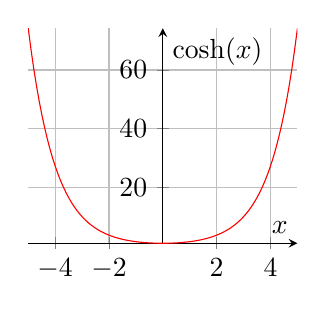
\begin{tikzpicture}
			\begin{axis}[domain=-5:5, axis lines=middle, grid=both, xlabel=$x$, ylabel=$\cosh(x)$, width=5cm]
				\addplot[color=red, samples=100]  {cosh(x)};
			\end{axis}
		\end{tikzpicture}
		\caption{Fonction cosh}
	\end{subfigure}
	\begin{subfigure}{0.3\textwidth}
		%\includegraphics[width=\textwidth, height=3.5cm]{images/sh.png}
		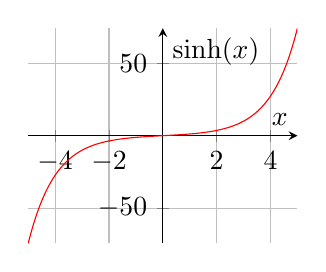
\begin{tikzpicture}
			\begin{axis}[domain=-5:5, axis lines=middle, grid=both, xlabel=$x$, ylabel=$\sinh(x)$, width=5cm]
				\addplot[color=red, samples=100]  {sinh(x)};
			\end{axis}
		\end{tikzpicture}
		\caption{Fonction sinh}
	\end{subfigure}
	\begin{subfigure}{0.3\textwidth}
		%\includegraphics[width=\textwidth, height=3.5cm]{images/tanh.png}
		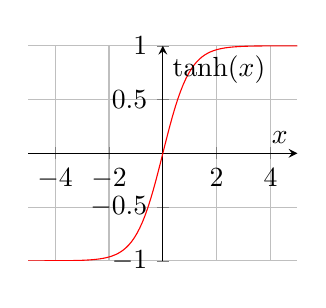
\begin{tikzpicture}
			\begin{axis}[domain=-5:5, axis lines=middle, grid=both, xlabel=$x$, ylabel=$\tanh(x)$, width=5cm]
				\addplot[color=red, samples=100]  {tanh(x)};
			\end{axis}
		\end{tikzpicture}
		\caption{Fonction tanh}
	\end{subfigure}
\end{figure}

\begin{proposition}
	Soit $x \in \R$.
	\begin{enumerate}
		\item $\cosh(-x) = \cosh(x)$.
		\item $\sinh(-x) = -\sinh(x)$.
		\item $\tanh(-x) = -\tanh(x)$.
	\end{enumerate}
\end{proposition}

\begin{proposition}
	Soient $x, y \in \R$.
    \begin{enumerate}
        \item $\cosh(x + y) = \cosh(x) \cosh(y) + \sinh(x) \sinh(y)$.
        \item $\sinh(x + y) = \cosh(x) \sinh(y) + \sinh(x) \cosh(y)$.
    \end{enumerate}
\end{proposition}

\begin{proof}
    Calcul direct avec les définitions de $\cosh$ et de $\sinh$.
\end{proof}

